\documentclass[12pt]{article}

\pagestyle{plain}
\oddsidemargin 0in       %   Left margin on odd-numbered pages.
\evensidemargin 0in        %   Left margin on even-numbered pages.
\textwidth 6.5in
\textheight 9in
\topmargin 0in
\headheight 0in
\headsep 0in

\usepackage[T1]{fontenc}
\usepackage{pslatex}
%\renewcommand*{\familydefault}{\sfdefault}

\usepackage{verbatim}
\newenvironment{qv}%
  {\quote
   \verbatim}%
  {\endverbatim
   \endquote}

\newcommand{\exx}{\\[2ex]}
\newcommand{\code}{\texttt}

\parskip 2ex
\parindent 0em


\begin{document}
\sloppypar

\begin{center}
\Large\bf
CIS 201 -- Computer Science I\\
Laboratory Assignment 4\\
\end{center}

\section*{Introduction}
In this lab you will create a game that will incorporate:
\begin{itemize}
\item selection (\code{if} and \code{if...else...} statements) 
\item boolean expressions
\item the \code{Color} class and customized colors
\item timed animations
\end{itemize}

\begin{comment}
\begin{figure}[htb]
  \begin{center}    
    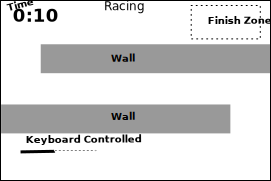
\includegraphics[width=6in]{Drawings/racing-design}  
    \caption{Racing Game Design}
  \label{fig:login}
  \end{center}
\end{figure}
\end{comment}


\section*{The \code{Racing} game}

Create a {\tt Lab04}
directory in your {\tt CS1} directory. In that directory, create a
Java file with a \code{Game} class named \code{Racing}.

Be sure to create an empty class template in the new file with a
header comment, an import statement, a class declaration,
and our standard two methods, as follows:


\begin{qv}
/**
 * Describe class Racing here.
 *
 *
 * Created: Aug. 3, 1978
 *
 * @author <a href="mailto:student1@potsdam.edu">Indiana Jones</a>
 * @author <a href="mailto:student2@potsdam.edu">Luke Skywalker</a>
 * @version 1.0
 */
import fang.core.Game;

public class Racing extends Game {
  /**
   * Describe setup method here
   */
  public void setup() {
    
  }
  
  /**
   * Describe advance method here
   * 
   * @param dT time (in fractional seconds) since the last call to advance
   */
  public void advance(double dT) {
    
  }
} // class Racing
\end{qv}

\section*{Add a car}

For this game, a car is simply a pie slice drawn on the screen. You
should add a \code{PieSprite} field to your game and, during setup,
construct it with the following parameters:
width=0.35, height=0.35, start=185.0, and end=195.0.
Locate the car at the point (0.1, 0.9).
If you want more details about how to construct a \code{PieSprite},
look it up in the FANG documentation.
Study the \code{NewtonsApple} code to see how to get things started.
You will need to give a variable name to the car you are creating.
What would be a good name for this variable??
The code to add a car should be in your \code{setup} method.
Be sure to use \code{addSprite} to add the car to the game canvas.

The car should be some shade of red. You can use the \code{getColor}
method to create a custom color if you call it with three integers
that represent the amount of the three primary colors
red, green, and blue. All three parameters are on the range 0..255;
all at 255 is white, all at 0 is black. Feel free to experiment a
little bit.  Use the value returned by \code{getColor}
to set the color of the car.

\subsection*{Checkpoint 1}
{\bf
Show us your working code at this point.
}

\section*{Add walls}

Add two long, thin rectangles that extend eighty percent of the way
across the screen, one from the right edge of the screen and one from
the left edge of the screen.
The right-edge wall should be about 1/3 from  the top
of the screen, and the other wall should be about 1/3 from the bottom.
These will be the walls that your car must avoid
as you ``drive'' the car from the bottom of the screen to the top.
Be sure that the walls give sufficient room for the car to turn around
and to get from the bottom of the game canvas to the top.

You should select your own custom colors using the \code{getColor} method
that expects three integers.  Make the top wall lightly colored, make
the bottom one darker, and make sure both are visible on the black
background of the game.

\subsection*{Checkpoint 2}
{\bf
Show us your working code at this point.
}

\section*{Make the car turn}

Part of what makes racing games fun is the need to steer.  Your racing
car moves one direction: straight ahead.  In its initial position, with
no rotation, it is pointing to the right.
You will need to write code to have the car
turn a small amount to the left or right
when the left or right arrow keys are pressed.

Looking at the \code{Sprite} documentation, you will see a method called
\code{rotateRevolutions}
(along with \code{rotateDegrees} and \code{rotateRadians}).
These methods turn the sprite
(in your case, the car)
by some amount.  If we knew how many revolutions the car
should turn per second, then we could use that value (just like we
did with our falling apples) inside of the \code{advance}
method to determine how much to rotate the car based
on the fraction \code{dT} of a second has elapsed.

In particular, if we have a variable \code{carTurningSpeed}
in revolutions per second,
then we would be able to
use something similar to what we did with the apple
and pass the scaled value (the speed times \code{dT}) to
\code{rotateRevolutions}.
For this game, you should set the car turning speed
to 0.5 revolutions per second.

Where will you declare the \code{carTurningSpeed} variable, and where
will you initialize it to 0.5?

Next, add a \emph{multi-way} \code{if} statement to \code{advance}
that will turn the car.
If the you press the left-arrow key, turn the car to the left;
if you press the right-arrow key, turn the car to the right.
What methods can you use to detect if the left- or right-arrow keys
have been pressed?

\subsection*{Checkpoint 3}
{\bf
Show us your working code at this point.
}

\section*{Move the car}

Now it is time to move the car. You will do exactly what you did to
move the apple, but instead of \code{translateY} or \code{translateX},
you will use the \code{forward} method of \code{Sprite}.
What does \code{forward} do? What parameter does it expect? Read the
documentation and see if you have questions.

If you press the up-arrow key, you should move the car forward with its
speed scaled by the time since the last \code{advance}. You will need
a variable to hold the car's speed; it should be about 0.25 screens/second.
The check for the up-arrow key should be part
of the same multi-way \code{if} you did above.

\subsection*{Checkpoint 4}
{\bf
Show us your working code at this point.
}

\section*{Timing}

Let's just keep track of elapsed time. We will start by adding a
field variable \code{elapsedTime} that is initialized to
\code{0.0}. Again, where should it be declared and where should it be
initialized?

The elapsed time also needs to be updated.
Since \code{advance} gets
called with the parameter \code{dT} equal
to the number of seconds since the last call,
you can update the elapsed time in \code{advance} by adding the time
since last call to your elapsed time variable.
However, you should update the elapsed time only if 
the game has not finished. How can you tell if a game
has finished?  Look at the documentation.

You also need a \code{StringSpirte} to display the elapsed
time. Initialize it properly and position it somewhere
inside the upper wall.
You will need to call the \code{scale()} method to make it fit.
Make an \code{updateTimer} method that
creates a string representing the elapsed time
as ``MM:SS'' where ``MM'' is the number of
minutes and ``SS'' is the number of seconds elapsed,
and that puts this string into the \code{StringSprite}.
The \code{setText} method of a \code{StringSprite}
allows you to determine what gets displayed in the sprite.

Problem: How do we get the number of minutes and seconds?
The \code{elapsedTime} variable is a double that gives you
the total number of elapsed seconds since the game started.
You will need to define a local integer variable
to hold the current number of minutes
and another local integer variable to hold
the number of seconds (which should be less than 60).

Assign the elapsed time to the seconds variable first --
you will need to use a cast to do this.
Then find the minutes by dividing the seconds by 60,
and finally modify the seconds to be the remainder upon division by 60.
The integer division and modulus operator (\verb'\%') should be used here:

\begin{qv}
int seconds = (int) elapsedTime;
int minutes = seconds / 60;
seconds = seconds % 60;
\end{qv}

Once you have the number of minutes and seconds,
you can set the text of the \code{StringSprite} to the
expression \code{minutes + ":" + seconds}.

\subsection*{Checkpoint 5}
{\bf
Show us your code at this point.
}

\section*{Crash}
Add crashing to the game. If the car hits either of the walls, it
should have its position and rotation set back to their initial
values. You may use only one \code{if} statement to handle collision
with either wall.
Suppose \code{car} is the race car and \code{wall1} is one of the walls.
The boolean expression
\begin{qv}
car.intersects(wall1)
\end{qv}
will return \code{true} if the car and the wall intersect,
and will return \code{false} otherwise.
What boolean expression should you use
to determine if the car intersects {\em either}
\code{wall1} or \code{wall2}?

If the car collides with either wall,
use \code{setLocation} and
\code{setRotation} to reset the car to the initial settings,
putting the car back at start.

Question: Should the collision detection be part
of the multi-way selection statement for the three arrow keys?

\subsection*{Checkpoint 6}
{\bf
Show us your work at this point.
}

\section*{The finish line}

You should check if the car has driven into the ``finish zone'' at the
upper right of the screen. You should do this in a single
\code{if} statement.
Check for winning only after you check for wall collision!

The finish zone is above your topmost wall to the top of the
screen. When the driver drives into the finish zone, turn the color of
the score to red and stop the game.

There are a couple ways to see if the car is in the finish zone.
The first would be to check the location of the car
(the \code{getX()} and \code{getY()} methods will do the trick)
and check to see if it's within the appropriate rectangle.
The other way is to create a ``finish zone'' rectangle sprite
that is colored black (so you don't see it)
and that occupies the finish zone.
Then the game is won if the car has intersected that rectangle.

When the user enters the finish zone, set the game to be over and turn
off the advancing of the timer. Setting the game to over is easy:
just call the \code{stop()} method.

\subsection*{Checkpoint 7}
{\bf
Show us your finished game.
}

\end{document}
